\documentclass[serif,xcolor=pdftex,dvipsnames,table,hyperref={bookmarks=false,breaklinks}]{beamer}

%%%%%%%%%%%%%%%%
% Change the macros below to configure the title slides
% for your course.
\newcommand{\coursename}{COMPSCI 589}
\newcommand{\instructor}{Benjamin M. Marlin}
\newcommand{\university}{University of Massachusetts Amherst}
\newcommand{\department}{College of Information and Computer Sciences}
%%%%%%%%%%%%%%%%


\newcommand{\settitlecard}[2]{
  \title[\coursename  Lecture #1] 
    {\coursename \\ Lecture #1: #2}
     \author[\instructor]{\instructor}
     \institute[\university]{
     \department\\
     \university
   }
\date{}
}

\newcommand{\maketitlepage}{
  \begin{frame}
  \titlepage
  \center{
    %If you use the slides unmodified, retain the attribution below
    \tiny{Slides by Benjamin M. Marlin (marlin@cs.umass.edu). \\
    \vspace{-1em}Created with support from National Science Foundation Award\# IIS-1350522. 
    %If you modify the slides, please retain the alternate attribution below
    %\tiny{Based on slides by Benjamin M. Marlin (marlin@cs.umass.edu). \\    
    %\vspace{-1em}Created with support from National Science Foundation Award\# IIS-1350522. 
    }                                              
  }  
  \end{frame}
}

\AtBeginSection[]
{
  \begin{frame}<beamer>{Outline}
    \tableofcontents[currentsection,subsectionstyle=hide]
  \end{frame}
}


\newcommand{\cut}[1]{}

\newcommand{\iconbox}[4]{
  \only<#1-#2>{
    \begin{columns}[T]
      \column{0.5in}
           \includegraphics[width=0.5in]{#3}
       \column{3.7in}
            #4
    \end{columns}
    \medskip
    \medskip
    \medskip
  }
}

\mode<presentation>{
  \usepackage{../beamertheme589theme}
  \setbeamercovered{invisible}
}

\mode<handout>{
  \usepackage{../beamertheme589theme}
  \setbeamercovered{transparent}
}


\usepackage[english]{babel}
\usepackage[latin1]{inputenc}
\usepackage{times}
\usepackage[T1]{fontenc}
\usepackage{amsmath}
\usepackage{amssymb}
\usepackage[noend]{algorithmic}
\usepackage{algorithm}
\usepackage{listings}

\renewcommand\mathfamilydefault{\rmdefault}

\newcommand{\setA}{\mathcal{A}}
\newcommand{\setB}{\mathcal{B}}
\newcommand{\setS}{\mathcal{S}}
\newcommand{\setV}{\mathcal{V}}
\DeclareMathOperator*{\union}{\bigcup}
\DeclareMathOperator*{\intersection}{\bigcap}
\DeclareMathOperator*{\Val}{Val}
\newcommand{\mbf}[1]{{\mathbf{#1}}}
\DeclareMathOperator*{\argmax}{arg\,max}
\DeclareMathOperator*{\argmin}{arg\,min}
\DeclareMathOperator*{\sign}{sign}
\newcommand{\deriv}[2]{\frac{\partial{#1}}{\partial{#2}}}


\settitlecard{19}{Principal Components Analysis}

\begin{document}

\maketitlepage

\section{Review}
\subsection{Foo}

\begin{frame}[t]{The Dimensionality Reduction Task}

\begin{block}{Definition: The Dimensionality Reduction Task}
Given a collection of feature vectors $\mbf{x}_i\in\mathbb{R}^D$, map the 
feature vectors into a lower dimensional space $\mbf{z}_i\in\mathbb{R}^K$ where 
$K<D$ while preserving certain properties of the data.
\end{block}

\pause
\center
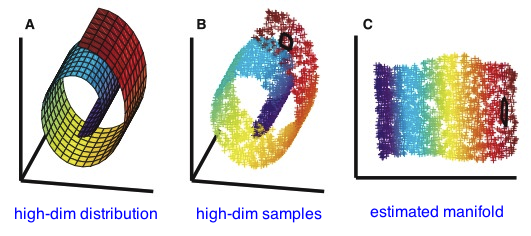
\includegraphics[width=4in]{../Figures/manifold_unrolling.png}
\end{frame}


\begin{frame}[t]{Linear Dimensionality Reduction}
 
\begin{itemize}
\item The simplest dimensionality reduction methods assume that the observed 
high dimensional data vectors $\mbf{x}_i\in \mathbb{R}^D$ lie on a 
K-dimensional linear manifold within $\mathbb{R}^D$. 

\item Mathematically, the linear sub-space assumption can be written as 
$\mbf{X} = \mbf{Z}\times \mbf{B}$

\center
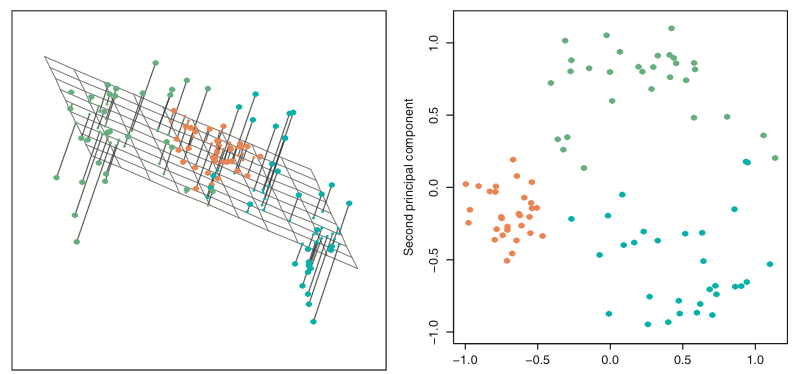
\includegraphics[width=3in]{../Figures/linear_subspace.png}


\end{itemize} 
\end{frame}

\begin{frame}[t]{Learning}
 
\begin{itemize}
\item The learning problem for linear dimensionality reduction is to estimate
values for both $\mbf{Z}$ and $\mbf{B}$ given only the noisy observations 
$\mbf{X}$.

\item One possible learning criteria is to minimize the sum of squared 
errors when reconstructing $\mbf{X}$ from $\mbf{Z}$ and $\mbf{B}$. This leads 
to:

{\Large
$$\argmin_{\mbf{Z},\mbf{B}} ||\mbf{X} - \mbf{Z}\mbf{B} ||_F$$
}

where $||\mbf{A}||_F$ is the Frobenius norm of matrix  $\mbf{A}$ (the sum of 
the squares of all matrix entries). 

\end{itemize} 
\end{frame}

\begin{frame}[t]{Singular Value Decomposition}
 
\begin{itemize}

\item We can pick a unique representation for the subspace by 
specifying additional criteria. Classical Rank-K Singular Value Decomposition 
(K-SVD) corresponds to the following restriction:

$$\argmin_{\mbf{U},\mbf{S},\mbf{V}} ||\mbf{X} - \mbf{U}\mbf{S}\mbf{V}^T ||_F$$

where $S$ is a $K\times K$ diagonal matrix with positive elements,  
$\mbf{U}$ is an $N\times K$ matrix such that  $\mbf{U}^T\mbf{U}=I$, and $V$
is a $DxK$ matrix such that $\mbf{V}^T\mbf{V}=I$.

\pause\item The matrix product $\mbf{Z}=\mbf{U}\mbf{S}$ gives the optimal 
rank-K representation of $\mbf{X}$ with respect to Frobenius norm minimization,
with $\mbf{V}^T$ acting as the basis for the space.

\end{itemize} 
\end{frame}

\section{Linear Algebra}
\subsection{foo}

\begin{frame}[t]{Eigenvectors}
 
\begin{itemize}

\item Let $\mbf{A}\in \mathbb{R}^{DxD}$ be a matrix, $\mbf{v}\in 
\mathbb{R}^{D}$ be a vector, and $\lambda$ be scalar.

\pause\item If $\mbf{A}\mbf{v} = \lambda \mbf{v}$ then $\mbf{v}$ is a right 
eigenvector of $A$ with eigenvalue $\lambda$.

\pause\item If $\mbf{A}^T\mbf{v} = \lambda \mbf{v}$ then $\mbf{v}$ is a 
left eigenvector of $A$ with eigenvalue $\lambda$ (equivalently 
$\mbf{v}^T\mbf{A} = \lambda \mbf{v}^T$).

\pause\item If $\mbf{A}$ is symmetric so that $\mbf{A}=\mbf{A}^T$, then the 
left and right eigenvectors of $\mbf{A}$ are the same with the same eigenvalues.

\pause
$$\begin{bmatrix}2&1\\1&2\end{bmatrix} 
\pause
\begin{bmatrix}1\\1\end{bmatrix} 
=\begin{bmatrix}3\\3\end{bmatrix}
=3\begin{bmatrix}1\\1\end{bmatrix}
$$

\pause
$$\begin{bmatrix}1 & 1\end{bmatrix} 
\begin{bmatrix}2 & 1\\ 1 & 2\end{bmatrix} 
=3\begin{bmatrix}1 & 1\end{bmatrix} 
$$

\pause\item A full-rank (invertible) matrix $\mbf{A}\in 
\mathbb{R}^{DxD}$ will have $D$ linearly independent eigenvectors.

\end{itemize} 
\end{frame}

\begin{frame}[t]{Eigendecomposition}
 
\begin{itemize}

\item Let $\mbf{V} \in \mathbb{R}^{DxD}$ be a matrix whose columns 
$\mbf{v}_d$ are $D$ linearly independent eigenvectors of $\mbf{A}$ 
with $\Lambda$ the corresponding diagonal matrix of eigenvalues such that 
$\Lambda_{dd}=\lambda_d$.Then:

{\Large
$$\mbf{A}\mbf{V} = \mbf{V}\Lambda$$
\pause
$$\mbf{A} = \mbf{V}\Lambda \mbf{V}^{-1}$$
\pause
$$\mbf{V}^{-1}\mbf{A}\mbf{V} = \Lambda $$
}

\pause\item Without loss of generality, we can assume that $\lambda_1\geq 
\lambda_2\geq  ... \geq \lambda_D$,

\end{itemize} 
\end{frame}


\begin{frame}[t]{Eigendecomposition of a Symmetric Matrix}
 
\begin{itemize}

\item If $\mbf{A}$ is symmetric, we can choose $D$ orthonormal eigenvectors so that
$||\mbf{v}_d||_2=1$, $\mbf{v}^T_d \mbf{v}_{d'}=0$ and $D$ real eigenvalues 
$\lambda_d\in \mathbb{R}$. This representation of $\mbf{A}$ is unique. 
As a result, we have:

{\Large
$$\mbf{A} = \mbf{V}\Lambda \mbf{V}^T = \sum_{d=1}^D \lambda_d \mbf{v}_d\mbf{v}^T_d$$

\pause
$$\mbf{V}^T\mbf{A}\mbf{V}=\Lambda$$ 
}

\end{itemize} 
\end{frame}

\begin{frame}[t]{Representation of a Vector in the Eigen Basis}
 
\begin{itemize}

\item Similarly, if $\mbf{a}$ is an arbitrary vector, then we can also 
represent $\mbf{a}$ using the basis provided by the eigevectors $\mbf{V}$ of a 
real symmetric matrix $\mbf{A}$. We obtain:

\Large
\begin{align}
\mbf{a} &= \sum_{d=1}^D \alpha_d \mbf{v}_d\\
\alpha_d&= \mbf{a}^T\mbf{v}_d
\end{align}

\end{itemize} 
\end{frame}


\begin{frame}[t]{Geometry}
 
\begin{itemize}

\item If $\mbf{A}$ is a real symmetric matrix with positive eigenvalues, then 
the quadratic equation $\mbf{x}^T\mbf{A}\mbf{x}=0$ defines an ellipsoid in a 
$D$-dimensional space, which provides a different way of thinking about these 
operations:

\pause
\center
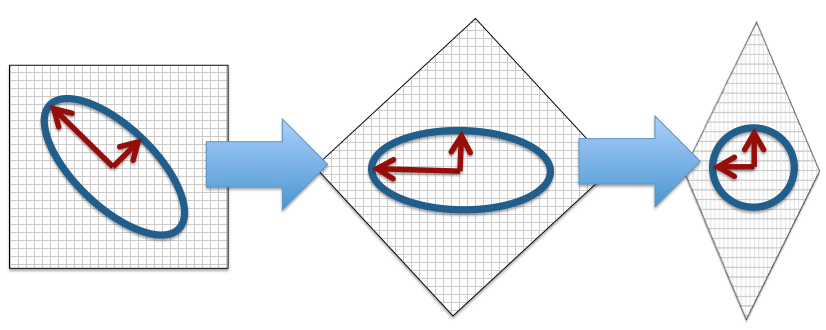
\includegraphics[width=4in]{../Figures/eigen_basis_change.png}

\end{itemize} 
\end{frame}

\section{PCA}
\subsection{foo}

\begin{frame}[t]{Principal Component Analysis}
 
\begin{itemize}
\item Given a data matrix $\mbf{X}\in \mathbb{R}^{N\times D}$, 
the goal of Principal Component Analysis (PCA) is to identify the directions
of maximum variance contained in the data.

\pause
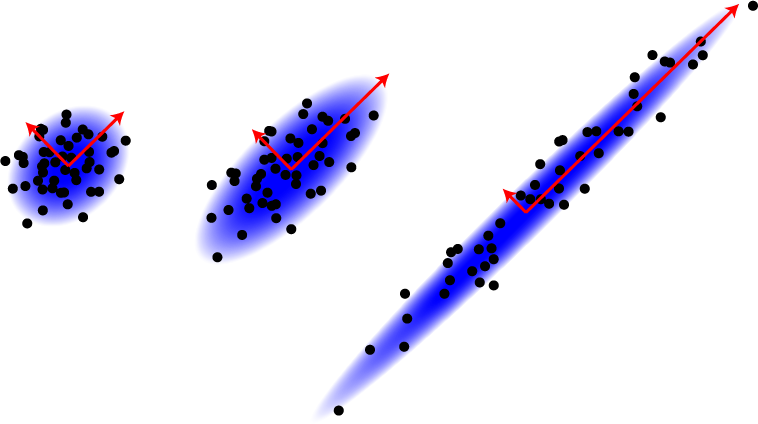
\includegraphics[width=4in]{../Figures/pca1.png}

\end{itemize} 
\end{frame}


\begin{frame}[t]{Sample Variance in a Given Direction}

\begin{itemize}
\item Let $\mbf{w}\in \mathbb{R}^{D}$ such that 
$||\mbf{w}||_2=\sqrt{\mbf{w}^T\mbf{w}}=1$. 

\pause\item The sample estimate of the variance in the direction 
$\mbf{w}$ given the data set $\mbf{X}$ is given by the expression:

$$ \frac{1}{N}\sum_{i=1}^N (\mbf{X}_i\mbf{w}-\mu)^2 \;\;\mbox{ where} \;\;
\mu = \frac{1}{N}\sum_{i=1}^N \mbf{X}_i\mbf{w}$$ 

\end{itemize} 
\end{frame}

\begin{frame}[t]{Pre-Centering}

\begin{itemize}
\item Under the assumption that the data are 
pre-centered so that $\frac{1}{N}\sum_{i=1}^N \mbf{X}_i=0$, this expression 
simplifies to:

\begin{align*}
\frac{1}{N}\sum_{i=1}^N (\mbf{X}_i\mbf{w})^2 
= (\mbf{X}\mbf{w})^T(\mbf{X}\mbf{w}) 
= \mbf{w}^T\mbf{X}^T\mbf{X}\mbf{w}
\end{align*}

\end{itemize} 
\end{frame}

\begin{frame}[t]{The Direction of Maximum Variance}

\begin{itemize}
\item Suppose we want to identify the direction $\mbf{w}_1$ of maximum variance 
given the data matrix $\mbf{X}$. We can formulate this optimization problem as 
follows:

\pause
\begin{align*}
\mbf{w}_1 = \max_{\mbf{w}} \mbf{w}^T\mbf{X}^T\mbf{X}\mbf{w} \mbox{ ... st } 
||\mbf{w}||_2=1
\end{align*}

\pause\item How can we solve this problem?

\end{itemize} 
\end{frame}

\begin{frame}[t]{The Direction of Maximum Variance}

\begin{itemize}
\item Let $\Sigma = \mbf{X}^T\mbf{X}$. 

\pause \item $\Sigma$ is real and symmetric, so it 
admits an eigendecomposition of the form: 
$$\Sigma = \sum_{d=1}^D \sigma_d 
\mbf{V}_d\mbf{V}_d^T$$

\pause \item $\sigma_1\geq \sigma_2 \geq,...,\geq \sigma_D\geq 0$ are the 
eigenvalues of $\Sigma$. 

\pause \item $\mbf{V}_d\in \mathbb{R}^D$ are the eigenvectors of $\Sigma$.
They satisfy: 

$$||\mbf{V}_d||_2 = \sqrt{\mbf{V}_d^T\mbf{V}_d} =1 \mbox{ ... for all } d$$ 

$$\mbf{V}_d^T\mbf{V}_{d'} =0 \mbox{ ... for all } d\neq d'$$ 

\end{itemize} 
\end{frame}

\begin{frame}[t]{The Direction of Maximum Variance}

\begin{itemize}
\item Using this result, we can write the optimization problem as:


$$\max_{\mbf{w}} \mbf{w}^T\mbf{X}^T\mbf{X}\mbf{w} \mbox{ ... st } 
||\mbf{w}||_2=1 $$
\pause
$$\max_{\mbf{w}} 
\mbf{w}^T\left(\sum_{d=1}^D \sigma_d \mbf{V}_d\mbf{V}_d^T\right)\mbf{w} \mbox{ 
... st } 
||\mbf{w}||_2=1$$
\pause
$$\max_{\mbf{w}} \sum_{d=1}^D \sigma_d 
(\mbf{w}^T\mbf{V}_d)^2 \mbox{ ... st } 
||\mbf{w}||_2=1 $$


\end{itemize} 
\end{frame}


\begin{frame}[t]{The Direction of Maximum Variance}

\begin{itemize}
\item $\mbf{w}$ can also be expressed in the orthonormal basis 
$\mbf{V}_1,...,\mbf{V}_D$ by letting $\mbf{w} = 
\sum_{d=1}^D\omega_d\mbf{V}_d$. 

\pause\item The constraint that $||\mbf{w}||_2=1 $ becomes $\sqrt{\sum_{d=1}^D 
\omega_d^2}=1$. 

\pause\item This means $\sum_{d=1}^D \omega_d^2=1$ and $\omega_d^2>0$, so the 
$\omega_d^2$ values act like a discrete probability distribution.

\end{itemize} 
\end{frame}


\begin{frame}[t]{The Direction of Maximum Variance}

\begin{itemize}

\item Plugging this back into the objective function, we have:

$$\max_{\mbf{w}} \sum_{d=1}^D \sigma_d 
(\mbf{w}^T\mbf{V}_d)^2 \mbox{ ... st } 
||\mbf{w}||_2=1 $$

\pause
$$\max_{\omega} \sum_{d=1}^D \sigma_d 
\left(\sum_{d'=1}^D\omega_{d'}\mbf{V}_{d'}^T\mbf{V}_d\right)^2 \mbox{ ... st } 
\sum_{d=1}^D \omega_d^2=1 $$

\pause
$$\max_{\omega} \sum_{d=1}^D \sigma_d \omega_d^2 \mbox{ ... st } 
\sum_{d=1}^D \omega_d^2=1 $$


\end{itemize} 
\end{frame}

\begin{frame}[t]{The Direction of Maximum Variance}

\begin{itemize}

\item At this point, the solution is clear.

\pause\item To maximize the variance, we need to set $\omega_1=1$ 
and set $\omega_d=0$ otherwise. \pause This put's all the weight on the maximum 
eigenvalue of $\Sigma$, which is $\sigma_1$ by assumption.

\pause\item Working our way back to $\mbf{w}_1$, we put all our weight on the 
maximum eigenvalue, so $\mbf{w} = 
\sum_{d=1}^D\omega_d\mbf{V}_d = \mbf{V}_1$.

\pause\item \textbf{This shows that the maximum variance direction given a data 
matrix $\mbf{X}$ is the eigenvector of $\mbf{X}^T\mbf{X}$ with the 
largest eigenvalue. }


\end{itemize} 
\end{frame}

\begin{frame}[t]{K Largest Directions of Variance}

\begin{itemize}

\item Suppose instead of just the direction of maximum variance, we want the 
$K$ largest directions of variance that are all mutually orthogonal.

\pause \item Finding the second-largest direction of variance corresponds to 
solving the problem:

\begin{align*}
\mbf{w}_2 &=  \max_{\mbf{w}} \sum_{d=1}^D \sigma_d 
(\mbf{w}^T\mbf{V}_d)^2 \mbox{ ... st } 
||\mbf{w}||_2=1 \mbox { and } \mbf{w}^T\mbf{w}_1=0
\end{align*}

\pause\item It's easy to see that this is going 
to be the eigenvector corresponding to the second largest eigenvalue.

\pause\item \textbf{In general, the top $K$ directions of variance 
$\mbf{w}_1,...,\mbf{w}_K$ are given by the $K$ eigenvectors corresponding to 
the $K$ largest eigenvalues of $\mbf{X}^T\mbf{X}$}.

\end{itemize} 
\end{frame}

\begin{frame}[t]{Dimensionality Reduction with PCA}

\begin{enumerate}
\item Given centered data matrix $\mbf{X} \in \mathbb{R}^{N\times D}$, compute 
unscaled sample covariance matrix $\Sigma = \mbf{X}^T\mbf{X}$.

\pause\item Compute the $K$ leading eigenvectors $w_1,...,w_K$ of $\Sigma$ 
where $\mbf{w}_k \in \mathbb{R}^D$.

\pause\item Stack the eigenvectors together into a $D \times K$ matrix 
$\mbf{W}$ where each column $k$ of $\mbf{W}$ corresponds to $\mbf{w}_k$.

\pause\item Project the matrix $\mbf{X}$ into the rank-K sub-space of maximum 
variance by computing the matrix product $\mbf{Z}=\mbf{X}\mbf{W}$.

\pause\item To reconstruct $\mbf{X}$ given $\mbf{Z}$ and $\mbf{W}$,
we use $\hat{\mbf{X}} = \mbf{Z}\mbf{W}^T$.

\end{enumerate} 
\end{frame}

\section{Connection to SVD}
\subsection{Foo}

\begin{frame}[t]{Connection to SVD}

\begin{itemize}
\item Last class we saw that the minimum Frobenius norm linear dimensionality 
reduction problem could be solved using the the rank-K SVD of $\mbf{X}$:

$$\argmin_{\mbf{U},\mbf{S},\mbf{V}} ||\mbf{X} - \mbf{U}\mbf{S}\mbf{V}^T ||_F$$

where the matrix product $\mbf{Z}=\mbf{U}\mbf{S}$ gives the optimal rank-K 
representation of $\mbf{X}$ with respect to Frobenius norm minimization.  


\end{itemize} 
\end{frame}


\begin{frame}[t]{Connection to SVD}

\begin{itemize}
\item If we let $K=D$ then $\mbf{X} = \mbf{U}\mbf{S}\mbf{V}^T$ and
$\mbf{X}^T\mbf{X} = \mbf{V}\mbf{S}\mbf{U}^T\mbf{U}\mbf{S}\mbf{V}^T$.

\pause\item Due to orthogonality of $U$ this gives: $\mbf{X}^T\mbf{X} = 
\mbf{V}\mbf{S}^2\mbf{V}^T$. 

\pause\item This means that the right singular vectors of 
$\mbf{X}$ are exactly the eigenvectors of $\mbf{X}^T\mbf{X}$, so 
SVD's $\mbf{V}$ and PCA's $\mbf{W}$ are identical (assuming $\mbf{X}$ is centered). 

\pause\item We can also see that the eigenvalues of $\mbf{X}^T\mbf{X}$ are the 
squares of the diagonal elements of $\mbf{S}$. 

\pause \item This means that the $K$ largest 
singular values and $K$ largest eigenvalues correspond to the same $K$ basis 
vectors.

\end{itemize} 
\end{frame}


\begin{frame}[t]{Connection to SVD}

\begin{itemize}

\item According to PCA, the projection operation is 
$\mbf{Z}=\mbf{X}\mbf{W}$. 

\pause\item Using $\mbf{X} = \mbf{U}\mbf{S}\mbf{V}^T$ and 
$\mbf{V}=\mbf{W}$ we have:

$$\mbf{Z}=\mbf{X}\mbf{W} = (\mbf{U}\mbf{S}\mbf{V}^T)(\mbf{V}) = \mbf{U}\mbf{S}$$ 

\pause\item Finally, note that if the decompositions are based only on the K 
leading basis vectors, which are identical under both PCA and SVD, the 
projections $\mbf{Z}=\mbf{X}\mbf{W}$ and $\mbf{Z}=\mbf{U}\mbf{S}$ will still be 
identical.

\end{itemize} 
\end{frame}

\begin{frame}[t]{Connection to SVD}

\begin{itemize}
\item These manipulations show that PCA on $\mbf{X}^T\mbf{X}$ and SVD on 
$\mbf{X}$ identify exactly the same sub-space and result in exactly the same 
projection of the data into that sub-space.

\pause\item As a result, generic linear dimensionality reduction 
simultaneously minimizes the Frobenius norm of the reconstruction error of 
$\mbf{X}$ and maximizes the retained variance in the learned sub-space.

\pause\item Both SVD and PCA provide the same refinement of generic linear 
dimensionality reduction: an orthogonal basis for exactly the same optimal 
linear subspace. 

\end{itemize} 
\end{frame}

\begin{frame}[t]{Issues}

\begin{itemize}
\item The computational complexity of PCA is $O(D^2N + D^3)$ if the full 
eigendecomposition is obtained and then truncated, compared to 
$O(min(DN^2, ND^2))$ for SVD.

\pause\item If $K<<D$, then PCA can also be computed iteratively, as can SVD.

\pause\item The basic SVD and PCA algorithms are not suitable for large-scale 
data. Instead, randomized algorithms are often used.

\pause\item The value of $K$ can sometimes be chosen based on looking for 
eigenvalue gaps in the eigenspectrum of the covariance matrix. Otherwise, a 
supervised end/side-task is needed or a criteria like AIC/BIC must be applied.

\end{itemize} 
\end{frame}

%Demo: http://cognitrn.psych.indiana.edu/nsfgrant/FaceMachine/faceMachine.html




\end{document}
